\documentclass[a4paper,12pt]{article}

\usepackage{graphicx}
\usepackage{caption}
\usepackage{subcaption}
\usepackage{tikz}
\usepackage{pgf}
\usepackage{amsmath}
\usetikzlibrary{arrows.meta}
\usepackage[utf8]{inputenc}
\usepackage[english,greek]{babel}
\usepackage{hyperref}

\title{Προσομοίωση και Μοντελοποίηση \newline Δυναμικών Συστημάτων \newline Εργασία 1}
\author{Ρουσομάνης Γεώργιος (ΑΕΜ: 10703)}
\date{Απρίλιος 2025}

\begin{document}

\maketitle

\section*{Εισαγωγή}
Σκοπός της εργασίας είναι η εκτίμηση αγνώστων παραμέτρων με χρήση της μεθόδου μέγιστης καθόδου και της 
μεθόδου σχεδίασης κατά \selectlanguage{english}Lyapunov\selectlanguage{greek} (παράλληλη και μικτή τοπολογία).
Οι μέθοδοι αυτοί ονομάζονται μέθοδοι πραγματικού χρόνου ή \selectlanguage{english}online\selectlanguage{greek}
γιατί δίνουν εκτίμηση μέσα σε χρόνο μιας δειγματοληψίας. Για την εκτίμηση αυτή, οι αλγόριθμοι πραγματικού 
χρόνου στηρίζονται στην τρέχουσα τιμή και στην αμέσως προηγούμενη, δουλεύουν δηλαδή αναδρομικά. Απευθύνονται
κυρίως σε εφαρμογές στις οποίες ο αλγόριθμος πρέπει να είναι υπολογιστικά απλός και η διαδικασία της εκτίμησης 
να ολοκληρωθεί πριν λάβει χώρα η επόμενη δειγματοληψία. Χαρακτηριστικά παραδείγματα τέτοιων εφαρμογών είναι ο 
προσαρμοστικός έλεγχος συστημάτων, η πρόβλεψη της απόκρισης συστημάτων, η ανίχνευση και αναγνώριση βλαβών σε 
δυναμικά συστήματα. Η εργασία επικεντρώνεται στην υλοποίηση των μεθόδων στο 
\selectlanguage{english}MATLAB\selectlanguage{greek}, την κατάλληλη επιλογή των παραμέτρων σύμφωνα με την 
λογική του \selectlanguage{english}trial and error\selectlanguage{greek} και την επίδραση του θορύβου στις
εκτιμήσεις.

\section*{Θέμα 1}
Το σύστημα που μελετούμε είναι το σύστημα μάζας-ελατηρίου-αποσβεστήρα με εξωτερική δύναμη, η εξίσωση του
οποίου δίνεται από τη σχέση:
\begin{equation}
    m \ddot{x}(t) + b \dot{x}(t) + k x(t) = u(t),
    \label{eq:system_ODE}
\end{equation}
όπου $x(t)$ \selectlanguage{english}[m]\selectlanguage{greek} η μετατόπιση, $m>0$ η μάζα, $b>0$ ένας σταθερός 
συντελεστής απόσβεσης, $k>0$ η σταθερά του ελατηρίου, και $u(t)$ η εξωτερική δύναμη. Θεωρούμε ότι οι πραγματικές
τιμές των παραμέτρων είναι $m=1.315$, $b=0.225$ και $k=0.725$. Θεωρούμε επίσης πως οι καταστάσεις $x(t)$, 
$\dot{x}(t)$ και η είσοδος $u(t)$ είναι μετρήσιμες. Θα εξετάσουμε τις περιπτώσεις όπου $u(t) = 2.5$ και 
$u(t) = 2.5\sin t$.

Πρώτο βήμα στην ανάλυσή μας είναι η προσομοίωση της απόκρισης του συστήματος με κάποια συνάρτηση 
\selectlanguage{english}ODE solver\selectlanguage{greek} του 
\selectlanguage{english}MATLAB\selectlanguage{greek}. Η παραπάνω ΔΕ περιγράφει ένα γραμμικό και χρονικά 
αμετάβλητο σύστημα (ΓΧΑ). Συνεπώς, μπορεί να αναπαρασταθεί από τις εξισώσεις κατάστασης:
\begin{equation}
\begin{aligned}
    \dot{x}(t) = A x(t) + B u(t) \\
    y(t) = C x(t) + D u(t)
\end{aligned}
\label{eq:state_space_equations}
\end{equation}
όπου εδώ $x(t)$ είναι το διάνυσμα καταστάσεων και $y$ η έξοδος του συστήματος.

Ξεκινώντας από την (\ref{eq:system_ODE}) έχουμε:
\begin{equation}
    \ddot{x}(t) = -\frac{b}{m} \dot{x}(t) -\frac{k}{m} x(t) + \frac{1}{m} u(t).
    \label{eq:system_ODE_2}
\end{equation}
Θέτοντας $x_1 = x(t)$ και $x_2 = \dot{x}(t)$, δηλαδή $\ddot{x}(t) = \dot{x}_2$, προκύπτει:
\begin{equation*}
\begin{aligned}
    &\dot{x}_1 = x_2 \\
    &\dot{x}_2 = -\frac{b}{m} x_2 -\frac{k}{m} x_1 + \frac{1}{m} u(t).
\end{aligned}
\end{equation*}
Θεωρώντας ως έξοδο $y$ την μετατόπιση $x(t)$, οι εξισώσεις κατάστασης γράφονται:
\begin{equation*}
\begin{aligned}
    \begin{bmatrix}
        \dot{x}_1 \\
        \dot{x}_2
    \end{bmatrix} &= 
    \begin{bmatrix}
        0 & 1 \\
        -\frac{b}{m} & -\frac{k}{m}
    \end{bmatrix} \cdot
    \begin{bmatrix}
        x_1 \\
        x_2
    \end{bmatrix} +
    \begin{bmatrix}
        0 \\
        \frac{1}{m}
    \end{bmatrix} u(t) \\
    y &= 
    \begin{bmatrix}
        1 & 0
    \end{bmatrix} \cdot
    \begin{bmatrix}
        x_1 \\
        x_2
    \end{bmatrix}
\end{aligned}
\end{equation*}
Άρα οι πίνακες $A, \, B, \, C, \, D$ είναι:
\begin{equation}
    A = 
    \begin{bmatrix}
        0 & 1 \\
        -\frac{k}{m} & -\frac{b}{m}
    \end{bmatrix}, \quad B = 
    \begin{bmatrix}
        0 \\
        \frac{1}{m}
    \end{bmatrix}, \quad C = 
    \begin{bmatrix}
        1 & 0
    \end{bmatrix}, \quad D = 0
    \label{eq:state_space_matrices}
\end{equation}
Για την επιλογή της κατάλληλης συνάρτησης \selectlanguage{english}ODE solver\selectlanguage{greek} είναι
σημαντικό να προσδιορίσουμε αν το σύστημά μας είναι άκαμτο ή μη-άκαμπτο. Η συνάρτηση μεταφοράς δίνεται από
τον τύπο:
\begin{equation*}
    H(s) = C(sI-A)^{-1}B + D
\end{equation*}
και με αντικατάσταση των πινάκων από την (\ref{eq:state_space_matrices}) παίρνουμε
\begin{equation}
    H(s) = \frac{1}{m} \frac{1}{s^2 + \frac{b}{m}s + \frac{k}{m}}
    \label{eq:transfer_function}
\end{equation}
Η γενική μορφή της συνάρτησης μεταφοράς δευτεροβάθμιου συστήματος δίνεται από:
\begin{equation}
    H(s) = \frac{\omega_n^2}{s^2 + 2 \zeta \omega_n + \omega_n^2}
    \label{eq:transfer_function_order_2}
\end{equation}
όπου $\omega_n$ η φυσική συχνότητα του συστήματος και $\zeta$ ο συντελεστής απόσβεσης.
Συγκρίνοντας τις σχέσεις (\ref{eq:transfer_function}) και (\ref{eq:transfer_function_order_2}) παίρνουμε:
\begin{equation*}
    \begin{aligned}
        &\omega_n = \sqrt{\frac{k}{m}} \\
        &\zeta = \frac{b}{2}\sqrt{\frac{1}{mk}}
    \end{aligned}
\end{equation*}
και με αντικατάσταση των $m=1.315$, $b=0.225$ και $k=0.725$ βρίσκουμε ότι $\omega_n = 0.7425$, 
$ \zeta = 0.1152$. Εφόσον ισχύει $\zeta < 1$ οι πόλοι του συστήματος είναι συζυγείς μιγαδικοί με σταθερά 
χρόνου $\tau = \frac{1}{\zeta \omega_n} = 11.7$ \selectlanguage{english}sec\selectlanguage{greek}. Επειδή
οι σταθερές χρόνου του συστήματος είναι της ίδιας τάξης μεγέθους, το σύστημα χαρακτηρίζεται ως μη-άκαμπτο.
Συνεπώς, επιλέγουμε την συνάρτηση \selectlanguage{english}ode45\selectlanguage{greek} με βήμα ολοκλήρωσης 
$dt = 0.01 < 2 \tau$.

\subsection*{Μέθοδος μέγιστης καθόδου}
Για την εκτίμηση των παραμέτρων $m$, $b$ και $k$ πρέπει αρχικά να φέρουμε το σύστημά μας σε γραμμικά
παραμετροποιήσιμη μορφή. Η (\ref{eq:system_ODE}) μπορεί να εκφραστεί ως:
\begin{equation}
    \ddot{x} = 
    \begin{bmatrix}
        \frac{b}{m} & \frac{k}{m} & \frac{1}{m}
    \end{bmatrix} \cdot
    \begin{bmatrix}
        -\dot{x} & -x & u
    \end{bmatrix}^T
    \label{eq:linearly_parameterized_form}
\end{equation}
Η παραπάνω εξίσωση περιέχει το $\ddot{x}$, το οποίο δεν είναι μετρήσιμο, γεγονός που καθιστά αδύνατη την άμεση 
εκτίμηση των παραμέτρων. Για να ξεπεράσουμε αυτό το πρόβλημα, θέτουμε $\ddot{x} = s^2x$ και εφαρμόζουμε 
και στα δύο μέλη το ευσταθές φίλτρο $\Lambda(s) = s^2 + \lambda_1 s + \lambda_2$. Τότε η εξίσωση 
(\ref{eq:linearly_parameterized_form}) μετασχηματίζεται ως εξής:
\begin{equation*}
    \begin{aligned}
        \frac{s^2}{\Lambda(s)}x &= 
        \begin{bmatrix}
            \frac{b}{m} & \frac{k}{m} & \frac{1}{m}
        \end{bmatrix} \cdot
        \begin{bmatrix}
            -\frac{\dot{x}}{\Lambda(s)} & -\frac{x}{\Lambda(s)} & \frac{u}{\Lambda(s)}
        \end{bmatrix}^T 
        \Rightarrow \\
        \left(1 - \frac{\lambda_1 s + \lambda_2}{\Lambda(s)}\right)x &= 
        \begin{bmatrix}
            \frac{b}{m} & \frac{k}{m} & \frac{1}{m}
        \end{bmatrix} \cdot
        \begin{bmatrix}
            -\frac{\dot{x}}{\Lambda(s)} & -\frac{x}{\Lambda(s)} & \frac{u}{\Lambda(s)}
        \end{bmatrix}^T 
        \Rightarrow \\
        x &= 
        \begin{bmatrix}
            \frac{b}{m} - \lambda_1 & \frac{k}{m} - \lambda_2 & \frac{1}{m}
        \end{bmatrix} \cdot
        \begin{bmatrix}
            -\frac{\dot{x}}{\Lambda(s)} & -\frac{x}{\Lambda(s)} & \frac{u}{\Lambda(s)}
        \end{bmatrix}^T 
    \end{aligned}
\end{equation*}
και περνώντας στο πεδίο του χρόνου:
\begin{equation}
    x(t) = \theta^{\star T}\phi(t)
    \label{eq:linearly_parameterized_form_2}
\end{equation}
όπου $\theta^{\star}$ είναι ένα άγνωστο σταθερό διάνυσμα που εμπεριέχει τις πραγματικές τιμές των παραμέτρων 
προς εκτίμηση και $\phi(t)$ το μετρήσιμο διάνυσμα οπισθοδρόμησης. Στόχος μας είναι η εύρεση μίας 
εκτίμησης $\hat{\theta}$ του $\theta^{\star}$ και έπειτα η εύρεση των εκτιμήσεων $\hat{m}$, $\hat{b}$, 
$\hat{k}$ για κάθε χρόνο $t$. Θεωρούμε το σύστημα αναγνώρισης:
\begin{equation}
    \hat{x}(t) = \hat{\theta}(t)\phi(t),
    \label{eq:identification_system}
\end{equation}
όπου η έξοδος $\hat{x}(t)$ αποτελεί εκτίμηση της εξόδου $x(t)$ του πραγματικού συστήματος 
(\ref{eq:linearly_parameterized_form_2}). Από τις (\ref{eq:linearly_parameterized_form_2}) και 
(\ref{eq:identification_system}) σχηματίζεται το σφάλμα αναγνώρισης:
\begin{equation}
    e = x - \hat{x} = x - \hat{\theta} \phi = (\theta^{\star} - \hat{\theta}) \phi
    \label{eq:identification_error}
\end{equation}
Η μέθοδος της μέγιστης καθόδου στηρίζεται για την εύρεση της αναδρομικής εκτίμησης $\hat{\theta}$ του 
$\theta^{\star}$ στην ελαχιστοποίηση ως προς $\hat{\theta}$ κατάλληλα ορισμένης συνάρτησης κόστους του $e$.
Η συνάρτηση κόστους που επιλέγουμε είναι:
\begin{equation}
    K(\hat{\theta}) = \frac{e^2}{2} = \frac{(x - \hat{\theta}\phi)^2}{2}.
    \label{eq:cost_function}
\end{equation}
Θέλουμε λοιπόν:
\begin{equation*}
    \arg \min_{\hat{\theta}} K(\hat{\theta}).
\end{equation*}
Η αναδρομική σχέση της νέας εκτίμησης $\hat{\theta}_{k+1}$ δίνεται από:
\begin{equation}
    \hat{\theta}_{k+1} = \hat{\theta}_k -\gamma \nabla K(\hat{\theta}) = 
    \hat{\theta}_k + \gamma(x - \hat{\theta}\phi)\phi = \hat{\theta}_k + \gamma e \phi,
    \quad \hat{\theta}(0) = \theta_0
    \label{eq:gradient_descend}
\end{equation}
όπου $\gamma > 0$ μία σταθερά, $\hat{\theta}(0)$ η αρχική τιμή του $\hat{\theta}$ και $\phi$, $e$ μετρήσιμα.
Έχοντας την εκτίμηση $\hat{\theta} = [\hat{\theta}_1\quad\hat{\theta}_2 \quad \hat{\theta}_3]^T$, τα
$\hat{m}, \, \hat{b}, \, \hat{k}$ προκύπτουν από τις σχέσεις:
\begin{equation*}
    \begin{aligned}
        \hat{m} = \frac{1}{\hat{\theta}_3}, \quad
        \hat{b} = \frac{\hat{\theta}_1 + \lambda_1}{\hat{\theta}_3}, \quad
        \hat{k} = \frac{\hat{\theta}_2 + \lambda_2}{\hat{\theta}_3}
    \end{aligned}
\end{equation*}

Θα μελετήσουμε την ευστάθεια του συστήματος (\ref{eq:identification_system}), (\ref{eq:gradient_descend}).
Για $m = 1.315$, $b = 0.225$, $k = 0.725$, το σύστημα (\ref{eq:system_ODE}) είναι ευσταθές, καθώς
οι πόλοι του βρίσκονται στο αριστερό ημιεπίπεδο. Επομένως, για φραγμένη είσοδο $u$, οι μεταβλητές κατάστασης
$x$ και $\dot{x}$ θα είναι επίσης φραγμένες, καθώς σχετίζονται γραμμικά με το $u$. Στην
(\ref{eq:linearly_parameterized_form_2}), το $\phi$ ορίζεται ως:
\begin{equation}
\phi = 
    \begin{bmatrix}
        -\frac{\dot{x}}{\Lambda(s)} & -\frac{x}{\Lambda(s)} & \frac{u}{\Lambda(s)}
    \end{bmatrix}^T. 
    \label{eq:regressor_vector}
\end{equation}
Εφόσον το $\Lambda(s)$ είναι ευσταθές φίλτρο και $x, \, \dot{x}, \, u \in L_{\infty}$ τότε θα ισχύει
$\phi \in L_{\infty}$. Παραγωγίζοντας την (\ref{eq:regressor_vector}) έχουμε:
\begin{equation}
\dot{\phi} = 
    \begin{bmatrix}
        -\frac{s}{\Lambda(s)}\dot{x} & -\frac{s}{\Lambda(s)}x & \frac{s}{\Lambda(s)}u
    \end{bmatrix}^T. 
    \label{eq:regressor_vector_derivative}
\end{equation}
Αφού το $\Lambda(s)$ είναι φίλτρο 2ης τάξης, ο βαθμός του αριθμητή της συνάρτησης μεταφοράς 
$\frac{s}{\Lambda(s)}$ θα είναι μικρότερος από τον βαθμό του παρανομαστή, άρα $\dot{\phi} \in L_{\infty}$.
Επομένως, σύμφωνα με το λήμμα \selectlanguage{english}Barbalat\selectlanguage{greek}, για εισόδους στην
(\ref{eq:linearly_parameterized_form_2}) που ικανοποιούν $\phi, \, \dot{\phi} \in L_{\infty}$, η 
(\ref{eq:gradient_descend}) εξασφαλίζει ότι η εκτιμώμενη έξοδος $\hat{x}(t)$ του συστήματος αναγνώρισης
$\hat{x}(t) = \hat{\theta}(t) u(t)$ θα συγκλίνει ασυμπτωτικά στην έξοδο $x(t)$ του πραγματικού συστήματος 
$x(t) = \theta^{\star}u(t)$, και ο ρυθμός μεταβολής των παραμέτρων $\dot{\hat{\theta}}(t)$ θα μειώνεται με τον
χρόνο και θα συγκλίνει ασυμπτωτικά στο μηδέν.

Στο Σχήμα~\ref{fig:identification_error} φαίνεται το σφάλμα αναγνώρισης $e(t)$, η πραγματική έξοδος του 
συστήματος $x(t)$ και η εκτίμησή της $\hat{x}(t)$, για $u(t) = 2.5$ με $\gamma = 10^{-5}$ (αριστερά) και για 
$u(t) = 2.5 \sin t$ με $\gamma = 10^{-3}$ (δεξιά). Παρατηρούμε ότι και στις δύο περιπτώσεις το σφάλμα 
μηδενίζεται μέσα σε εύλογο χρονικό διάστημα. Όπως έχει ήδη εξηγηθεί, η σύγκλιση του $\hat{x}(t)$ στο 
$x(t)$ είναι εγγυημένη, καθώς και στις δύο περιπτώσεις ισχύει $u, \, \dot{u} \in L_{\infty}$, άρα 
$\phi, \, \dot{\phi} \in L_{\infty}$.

\begin{figure}[h!]
    \centering
    \begin{subfigure}{0.45\textwidth}
        \centering
        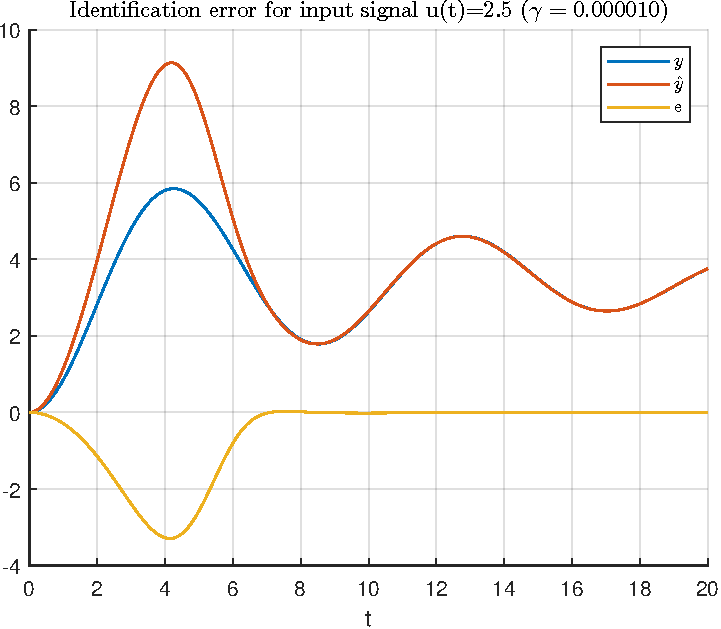
\includegraphics[width=\linewidth]{plot/identification_error_1.pdf}
        \caption{}
        \label{fig:identification_error_1}
    \end{subfigure}
    \hfill
    \begin{subfigure}{0.45\textwidth}
        \centering
        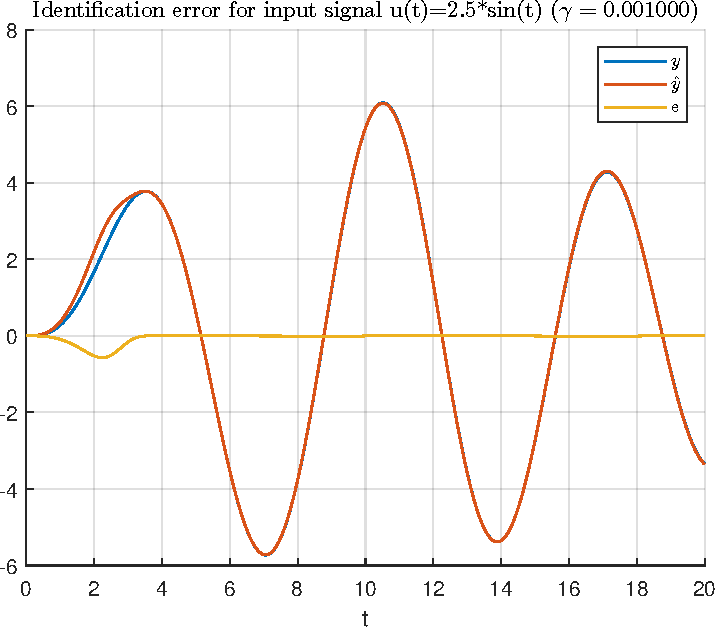
\includegraphics[width=\linewidth]{plot/identification_error_2.pdf}
        \caption{}
        \label{fig:identification_error_2}
    \end{subfigure}
    \caption{Σφάλμα αναγνώρισης για α) $u(t) = 2.5$ και β) $u(t) = 2.5 \sin t$}
    \label{fig:identification_error}
\end{figure}

Στο Σχήμα~\ref{fig:parameter_estimations} φαίνονται οι εκτιμήσεις των παραμέτρων για $u(t) = 2.5$ με 
$\gamma = 10^{-5}$ (αριστερά) και για $u(t) = 2.5 \sin t$ με $\gamma = 10^{-3}$ (δεξιά). Παρατηρούμε ότι και
στις δύο περιπτώσεις ο ρυθμός μεταβολής των παραμέτρων $\dot{\hat{\theta}}(t)$ μειώνεται με τον χρόνο, όπως 
άλλωστε αναμέναμε από το λήμμα \selectlanguage{english}Barbalat\selectlanguage{greek}. Επίσης, διαπιστώνουμε 
ότι για $u(t) = 2.5$ οι εκτιμήσεις των $m$ και $k$ απέχουν από τις πραγματικές τιμές τους κατά κάποια σταθερή 
ποσότητα. Αυτό μας προϊδεάζει ότι, ίσως σε αυτή την περίπτωση, το $\phi(t)$ δεν ικανοποιεί τη ΣΕΔ. Αντιθέτως,
για $u(t) = 2.5 \sin t$, οι εκτιμήσεις των παραμέτρων τείνουν ασυμπτωτικά να γίνουν ίσες με τις πραγματικές 
τιμές, κάτι που αποτελεί ένδειξη ότι το $\phi(t)$ ικανοποιεί τη ΣΕΔ.

\begin{figure}[h!]
    \centering
    \begin{subfigure}{0.45\textwidth}
        \centering
        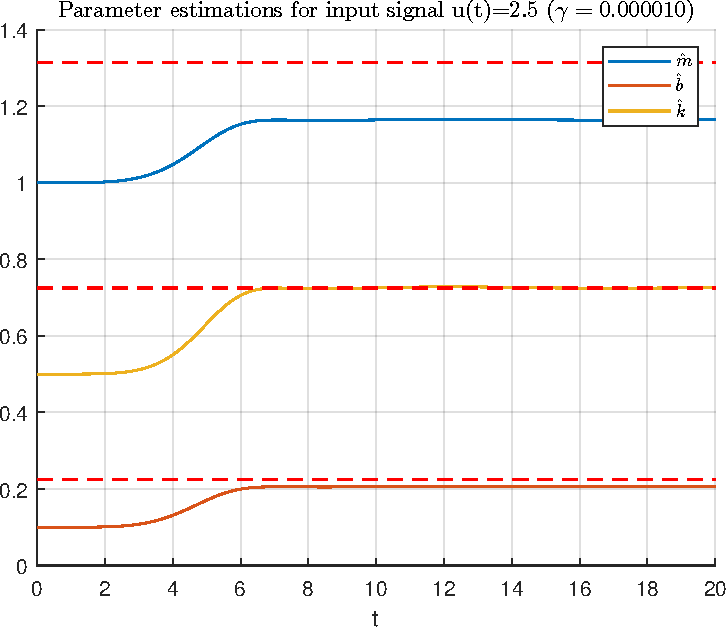
\includegraphics[width=\linewidth]{plot/parameter_estimations_1.pdf}
        \caption{}
        \label{fig:parameter_estimations_1}
    \end{subfigure}
    \hfill
    \begin{subfigure}{0.45\textwidth}
        \centering
        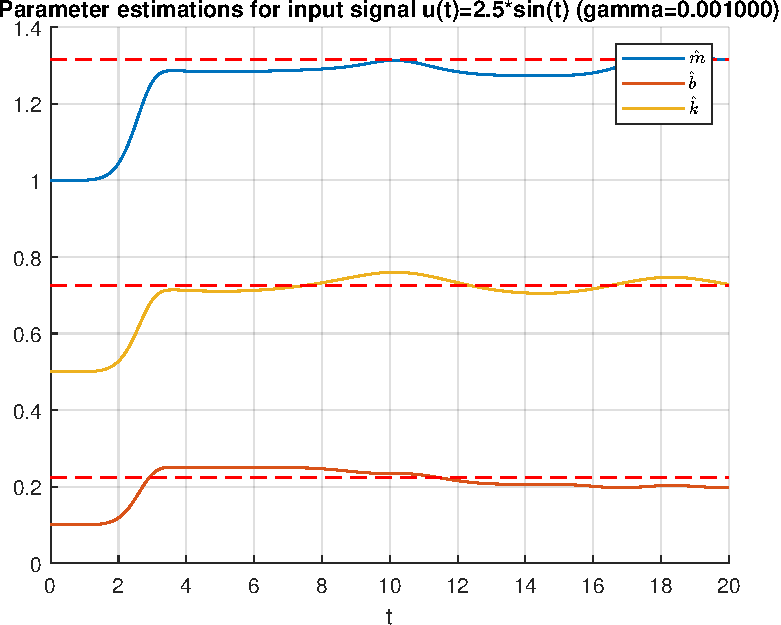
\includegraphics[width=\linewidth]{plot/parameter_estimations_2.pdf}
        \caption{}
        \label{fig:parameter_estimations_2}
    \end{subfigure}
    \caption{Εκτιμήσεις παραμέτρων για α) $u(t) = 2.5$ και β) $u(t) = 2.5 \sin t$}
    \label{fig:parameter_estimations}
\end{figure}

Θα εξετάσουμε αν το διάνυσμα $\phi(t)$ ικανοποιεί τη ΣΕΔ για τις δύο περιπτώσεις εισόδου. Λέμε ότι το διάνυσμα 
$\phi(t)$ ικανοποιεί τη Συνθήκη Εναπομείνουσας Διέγερσης (ΣΕΔ) με επίπεδο διέγερσης $\alpha_0 > 0$, αν
υπάρχουν σταθερές $\alpha_1, \, T_0 > 0$ τέτοιες ώστε:
\begin{equation}
    \alpha_1 I \ge \frac{1}{T_0} \int_{t}^{t+T_0} \phi(\tau) \phi^T(\tau) d\tau \ge \alpha_0 I, 
    \quad \forall t \ge 0
    \label{eq:PE}
\end{equation}
με $I$ τον μοναδιαίο πίνακα.

Όπως φαίνεται από την (\ref{eq:regressor_vector}), η μορφή του $\phi$ δεν επιτρέπει τον εκ των προτέρων
έλεγχο ικανοποίησης της (\ref{eq:PE}), γνωρίζοντας την είσοδο $u(t)$. Πρέπει δηλαδή εκ του αποτελέσματος να 
διαπιστώσουμε την ικανοποίηση της συνθήκης αυτής, άρα και τη σύγκλιση του $\hat{\theta}$ στο $\theta^{\star}$.

Στο Σχήμα~\ref{fig:PE_eigenvalues_1} φαίνονται οι ιδιοτιμές του πίνακα 
$\int_{t}^{t+T_0} \phi(\tau) \phi^T(\tau) d\tau$ για $u(t) = 2.5$. Βλέπουμε ότι μία εκ των τριών ιδιοτιμών δεν
έχει άνω φράγμα, άρα η ΣΕΔ δεν ικανοποιείται, κάτι που συμφωνεί με τις παρατηρήσεις μας για το 
Σχήμα~\ref{fig:parameter_estimations_1}.

Στο Σχήμα~\ref{fig:PE_eigenvalues_2} φαίνονται οι ιδιοτιμές του πίνακα 
$\int_{t}^{t+T_0} \phi(t) \phi(t)^T dt$ για $u(t) = 2.5 \sin t$. Σε αυτή την περίπτωση, βλέπουμε ότι όλες οι 
ιδιοτιμές είναι φραγμένες $\forall t \ge 0$, άρα ικανοποιείται η ΣΕΔ, κάτι που συμφωνεί με τα σχόλιά μας 
για το Σχήμα~\ref{fig:parameter_estimations_2}. 

Βλέπουμε επομένως ότι η ενέργεια του σήματος εισόδου $u(t) = 2.5 \sin t$ είναι τέτοια που να ενεργοποιεί με 
επειμένοντα τρόπο το σύστημα ώστε να μπορέσει να εμφανίσει την κρυμμένη πληροφορία $\theta^{\star}$.

\begin{figure}[h!]
    \centering
    \begin{subfigure}{0.45\textwidth}
        \centering
        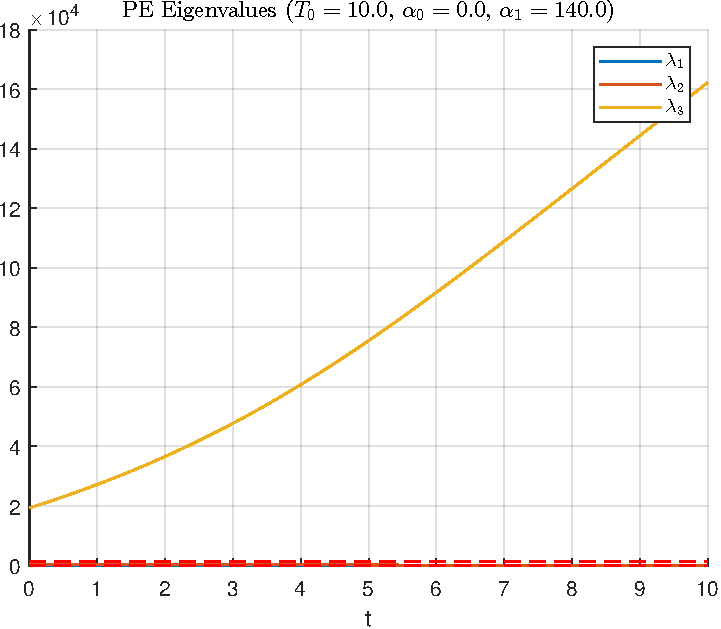
\includegraphics[width=\linewidth]{plot/PE_eigenvalues_1.pdf}
        \caption{}
        \label{fig:PE_eigenvalues_1}
    \end{subfigure}
    \hfill
    \begin{subfigure}{0.45\textwidth}
        \centering
        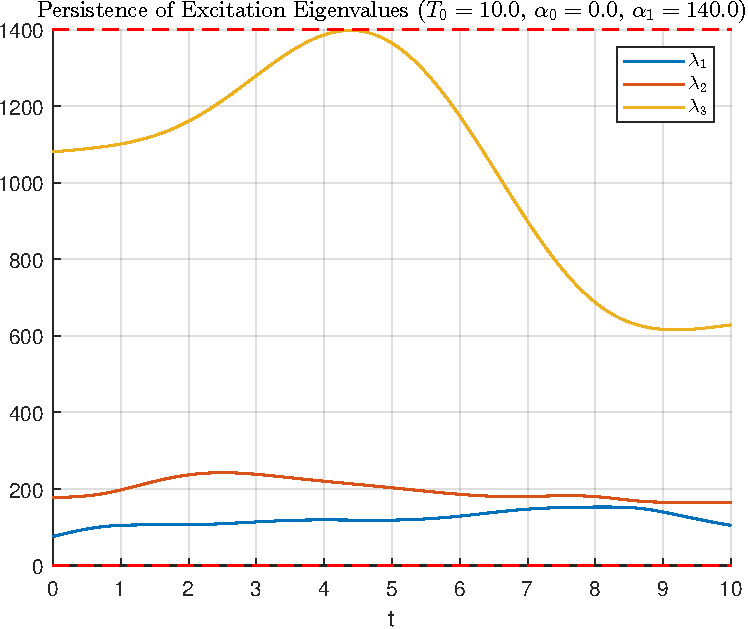
\includegraphics[width=\linewidth]{plot/PE_eigenvalues_2.pdf}
        \caption{}
        \label{fig:PE_eigenvalues_2}
    \end{subfigure}
    \caption{Ιδιοτιμές πίνακα $\int_{t}^{t+T_0} \phi(\tau) \phi^T(\tau) d\tau$ για 
    α) $u(t) = 2.5$ και β) $u(t) = 2.5 \sin t$}
    \label{fig:PE_eigenvalues}
\end{figure}

Στην (\ref{eq:gradient_descend}), η επιλογή του $\gamma$ έγινε με τη μέθοδο \selectlanguage{english}trial and 
error\selectlanguage{greek}. Γνωρίζουμε ότι όταν ισχύει η ΣΕΔ, αυξάνοντας την τιμή του $\gamma$, επιτυγχάνουμε 
ταχύτερη σύγκλιση του $\hat{\theta}(t)$ στο $\theta^{\star}$. Πολύ μεγάλες τιμές του $\gamma$, όμως, καθιστούν 
την (\ref{eq:gradient_descend}) άκαμπτη και επομένως δύσκολα αριθμητικά επιλύσιμη. Συνεπώς, οι τιμές του 
$\gamma$ επιλέχθηκαν ως οι μέγιστες δυνατές που δεν καθιστούν την (\ref{eq:gradient_descend}) άκαμπτη.

Στην ανάλυση που προηγήθηκε, φιλτράραμε το μη μετρίσιμο $\ddot{x}(t)$ με ένα ευσταθές φίλτρο 2ης τάξης. Αν 
χρησιμοποιούσαμε ένα ευσταθές φίλτρο 1ης τάξης, θα καταλήγαμε στη γραμμικά παραμετροποιήσιμη μορφή
$\dot{x}(t) = \theta^{\star T} \phi(t)$. Τότε το σύστημα αναγνώρισης θα ήταν 
$\hat{\dot{x}}(t) = \hat{\theta}(t)\phi(t)$ και το σφάλμα αναγνώρισης $e = \dot{x} - \hat{\dot{x}}$. 
Επομένως, σε αυτή την περίπτωση, η μέθοδος μέγιστης καθόδου θα μας έδινε την εκτίμηση $\hat{\theta}$ για την 
οποία η απόκλιση του $\hat{\dot{x}}$ από το $\dot{x}$ θα ήταν ελάχιστη.

\end{document}
